\section{Introduction}
The dynamics of a shaft in three systems is considered:
\begin{itemize}
    \item (I) Only shaft
    \item (II) Shaft and \SI{100}{\milli \meter} disc
    \item (III) Shaft, \SI{100}{\milli \meter} and \SI{80}{\milli \meter} discs
\end{itemize}
Both the unsupport shaft and the shaft supported by ball bearing and hydrodynamic bearing are considered. The dimensions of the shaft and discs is given in \cite[Appendix]{Problem}.
The shaft and both discs is made in ST60 steel with mechanical properties shown in table \ref{tab:mech_prop}.
\begin{table}[htbp]
    \centering
    \caption{Mechanical Properties of ST60 Steel}
    \label{tab:mech_prop}
    \begin{tabular}{@{}cccc@{}}
        \toprule
        Density                                     &   Poisson Ratio   &   Elastic Modulus         &   Yield Strength \\ \midrule
        \SI{7800}{\kilo \gram \per \cubic \meter} &   0.3             &   \SI{200}{\giga \pascal} &   \SI{390}{\mega \pascal}                               \\ \bottomrule
    \end{tabular}
\end{table}

\section{Lateral Dynamics of Flexible Shaft}
The first step is creating a model of the shaft. The model is compared to a experimental result and adjusted accordingly.

\subsection{Modelling}
From the technical drawings in \cite[Appendix]{Problem} the shaft can be modelled and analyzed.

\subsubsection{Mechanical model}
The shaft is drawn in solidworks to calculate the mass and moment of inertia. When doing so some simplifications are done.
The keyways at the ends of the shafts are neglected and the small fillets are not included. Other small features, namely the screw hole at the end and the two small flanges on the shaft is likewise neglected.
The resulting geometry is perfectly balanced with the mass and moment of inertia shown in table \ref{tab:shaft_mass_moment}.
\begin{table}[htbp]
    \centering
    \caption{Mass and Moment of Inertia of Shaft}
    \label{tab:shaft_mass_moment}
    \begin{tabular}{@{}cc@{}}
        \toprule
        Mass                    &   Moment of Inertia                       \\ \midrule
        \SI{0.5}{\kilo \gram}   &   \SI{0.0001}{\kilo \gram \square \meter} \\ \bottomrule
    \end{tabular}
\end{table}

Other assumptions:

\subsubsection{Mathematical model}
3 mathematical models are discretized from the mechanical model with increasing number of elements. The coarse model is seen a as a shaft with constant diameter of \SI{90}{\milli \meter} and length of \SI{1150}{\milli \meter}. The coarse model is discretized into 18 equal length elements.
The fine model have more complex geometry. Here the shaft is broken up into 6 section with varying diameter and length, each with one element. This includes more of the intrecasiess of the orginal geometry.
The Very fine model have the same 6 sections as the fine model, but discretizes the sections with more elements. The very fine mesh consist of 17 elements in total.

\subsubsection{Undamped natural frequencies}
To calculate the undamped natural frequencies of the shaft the three mathematical models are used. To make the system solveable a very small bearing stiffnes of \SI{0.01}{\pascal} is added.

\subsubsection{Convergence}
To compare the three mathematical models, a convergence study is done. Here the 4 lowest (non rigid body) natural frequencies are compared.
The resulting natural frequencies are shown in table \ref{tab:natural_freq}.
\begin{table}[htbp]
    \centering
    \caption{Undamped Natural Frequencies of Shaft}
    \label{tab:natural_freq}
    \begin{tabular}{@{}cccc@{}}
        \toprule
        Mode    &   Coarse Model (\si{\hertz})    &   Fine Model (\si{\hertz})  &   Very Fine Model (\si{\hertz}) \\ \midrule
        1       &   303.9   &   392.9   &   371.4   \\
        2       &   828.5   &   1066.2  &   916     \\
        3       &   1601.5  &   1786.4  &   1612.2  \\
        4       &   2602.7  &   3660.2  &   2550.7  \\ \bottomrule
    \end{tabular}
\end{table}

\subsection{Validation}
The experimental results from \cite[6]{Problem} is compared to the mathematical model. The experimantal natural frequencies and the discrepancy between the 3 mathematical models and the experimental results is shown in table \ref{tab:validation}.

\begin{table}[htbp]
    \begin{adjustwidth}{-1cm}{-1cm}
    \centering
    \caption{Validation of Mathematical Model}
    \label{tab:validation}
    \begin{tabular}{@{}ccccc@{}}
        \toprule
        Mode    &   Experimental (\si{\hertz})    &   Coarse Model (\si{\percent})    &   Fine Model (\si{\percent})  &   Very Fine Model (\si{\percent}) \\ \midrule
        1       &   388     &   21.7   &   -1.3   &   4.3   \\
        2       &   930     &   10.9   &   -14.7  &   1.5     \\
        3       &   1689    &   5.2  &   -5.8  &   4.6  \\
        4       &   2624    &   0.8  &   -39.5  &   2.8  \\ \bottomrule
    \end{tabular}
    \end{adjustwidth}
\end{table}


\subsection{Model adjustment}
As the very fine model is within \SI{5}{\percent} of the experimental results, this model is deemed accurate enough for further analysis. This model is choosen for further analysis and is refered to as system (I)

\section{Lateral Dynamics of Flexible Shaft and Discs}
The next step is to add the discs to the shaft. The same procedure as before is done. First the \SI{80}{\milli \meter} disc is added and then the \SI{100}{\milli \meter} disc is added.

\subsection{Modelling}
As before the discs are drawn in solidworks to calculate the mass and moment of inertia. The resuting geometry is perfectly balanced with the mass and moment of inertia shown in table \ref{tab:disc_mass_moment}.

\subsubsection{Mechanical model}
\begin{table}[htbp]
    \centering
    \caption{Mass and Moment of Inertia of Discs}
    \label{tab:disc_mass_moment}
    \begin{tabular}{@{}ccc@{}}
        \toprule
        Disc diamter    &   Mass                    &   Moment of Inertia                       \\ \midrule
        \SI{80}{\milli \meter}\SI{0.5}{\kilo \gram}   &   \SI{0.0001}{\kilo \gram \square \meter} \\ 
        \SI{100}{\milli \meter} &   \SI{0.4}{\kilo \gram}   &   \SI{0.001}{\kilo \gram \square \meter}\\ \bottomrule
    \end{tabular}
\end{table}

The discs are assumed to be perfectly balanced. The internal details of the discs are neglected.
The model is assumed rigid with only rigid body motion. 

\subsubsection{Mathematical model - one disc}
The mass and moment of inertia of the \SI{100}{\milli \meter} disc is added to the mathematical model of the shaft, in the node corresponding to the placement seen in \cite[Appendix]{Problem}.
As the disc is assumed to be rigid the extra stifness of the disc is not added.

The natural frequencies of the system is calculated and shown in table \ref{tab:natural_freq_one_disc}.
\begin{table}[htbp]
    \centering
    \caption{Undamped Natural Frequencies of Shaft and One Disc}
    \label{tab:natural_freq_one_disc}
    \begin{tabular}{@{}cc@{}}
        \toprule
        Mode    &   Natural Frequency (\si{\hertz})    \\ \midrule
        1       &   288.8   \\
        2       &   596.5   \\
        3       &   1243.5  \\
        4       &   1852.1  \\ 
        5       &   2.283.5 \\ \bottomrule
    \end{tabular}
\end{table}


This model is refered to as system (II)

\subsubsectionmark{Mathematical model - two discs}
The mass and moment of inertia of the \SI{100}{\milli \meter} disc is added to the mathematical system (II) in the node corresponding to the placement seen in \cite[Appendix]{Problem}.
The disc is assumed to be rigid and the extra stifness of the disc is not added.

The natural frequencies of the system is calculated and shown in table \ref{tab:natural_freq_two_discs}.
\begin{table}[htbp]
    \centering
    \caption{Undamped Natural Frequencies of Shaft and Two Discs}
    \label{tab:natural_freq_two_discs}
    \begin{tabular}{@{}cc@{}}
        \toprule
        Mode    &   Natural Frequency (\si{\hertz})    \\ \midrule
        1       &   242.5   \\
        2       &   502.4   \\
        3       &   929.8  \\
        4       &   1262.9  \\ 
        5       &   2276.9 \\ \bottomrule
    \end{tabular}
\end{table}

This model is refered to as system (III)

\subsection{Validation}
With the natural frequencies of the systems (II) and (III) the experimental results from \cite[6]{Problem} is compared. The experimantal natural frequencies and the discrepancy between the mathematical models and the experimental results is shown in table \ref{tab:validation_two_discs}.
\begin{table}[htbp]
    \begin{adjustwidth}{-1cm}{-1cm}
    \centering
    \caption{Validation of Mathematical Model}
    \label{tab:validation_two_discs}
    \begin{tabular}{@{}ccccc@{}}
        \toprule
        Mode    &   Experimental (\si{\hertz})    &   System (II) (\si{\percent})    &   System (III) (\si{\percent})  \\ \midrule
        1       &   241     &   4       &   -0.6    \\
        2       &   498     &   10.8    &   -0.9    \\
        3       &   708     &   7.8     &   -31.3   \\
        4       &   1250    &   7.2     &   -1      \\ 
        5       &   2350    &   4.2     &   3       \\ \bottomrule
    \end{tabular}
    \end{adjustwidth}
\end{table}

A major discrepancy is seen in the third mode of system (III). This is due to an interaction between the two discs. The model is adjusted to account for this.

\subsection{Model adjustment}
As only one natural frequency is significantly off, both models is deemed accurate enough for further analysis.


\section{Modelling of Ball Bearing}
When including the ball bearings at the specified points on the shaft, system (I) is considered with the ball bearing stifness going from \SIrange{e1}{10e9}{\pascal}.
The 8 first natural frequencies compared with the stifnees can be seen on figure \ref{fig:ball_bearing_stiffness}.
\begin{figure}[htbp]
    \centering
    \begin{tikzpicture}

\begin{axis}[%
width=0.9\linewidth,
height=0.6\linewidth,
xmode=log,
ymode=log,
xlabel={Stiffness [\si{\newton \per \square \meter}]},
ylabel={Eigenfrequency [\si{\hertz}]},
grid=major,
legend pos=south east,
]
\addplot []
  table[row sep=crcr]{%
10	0.558817169537322\\
100	1.76716900355551\\
1000	5.58827870662501\\
10000	17.6715970158956\\
100000	55.879562490757\\
1000000	176.613998439708\\
10000000	555.56285341882\\
100000000	1489.30744562933\\
1000000000	1616.49133852598\\
};
\addlegendentry{1}

\addplot [color=red]
  table[row sep=crcr]{%
10	0.905483025557055\\
100	2.86338849220888\\
1000	9.05476056401027\\
10000	28.6314938158507\\
100000	90.4719654351087\\
1000000	283.9222647486\\
10000000	830.038370073486\\
100000000	1663.06489217114\\
1000000000	3259.85266871539\\
};
\addlegendentry{2}

\addplot [color=blue]
  table[row sep=crcr]{%
10	2333.65180752057\\
100	2333.65333036973\\
1000	2333.66855900639\\
10000	2333.82085866914\\
100000	2335.345179351\\
1000000	2350.71877075002\\
10000000	2515.18902486417\\
100000000	3932.52102629454\\
1000000000	7063.0111266213\\
};
\addlegendentry{3}

\addplot [color=green]
  table[row sep=crcr]{%
10	5755.27680532091\\
100	5755.27748269065\\
1000	5755.28425635248\\
10000	5755.35199440482\\
100000	5756.02951901966\\
1000000	5762.81914536959\\
10000000	5832.13233188595\\
100000000	6622.14946572135\\
1000000000	9716.37500170846\\
};
\addlegendentry{4}

\addplot [color=purple]
  table[row sep=crcr]{%
10	10127.4544127093\\
100	10127.4546794837\\
1000	10127.4573471899\\
10000	10127.4840248031\\
100000	10127.7508468415\\
1000000	10130.4236700464\\
10000000	10157.6171130726\\
100000000	10480.3164842834\\
1000000000	14149.0154727874\\
};
\addlegendentry{5}

\addplot [color=orange]
  table[row sep=crcr]{%
10	16019.1003535951\\
100	16019.1004920402\\
1000	16019.1018765057\\
10000	16019.1157211188\\
100000	16019.2541811847\\
1000000	16020.6401605633\\
10000000	16034.6390047921\\
100000000	16189.7635301771\\
1000000000	19796.3836166394\\
};
\addlegendentry{6}

\addplot [color=cyan]
  table[row sep=crcr]{%
10	22964.4386460796\\
100	22964.4387014646\\
1000	22964.439255301\\
10000	22964.4447938927\\
100000	22964.5001807139\\
1000000	22965.0541637429\\
10000000	22970.6055171908\\
100000000	23027.3181513416\\
1000000000	23809.3940691991\\
};
\addlegendentry{7}

\addplot [color=purple]
  table[row sep=crcr]{%
10	30342.7931571478\\
100	30342.7931709179\\
1000	30342.7933084283\\
10000	30342.7946834812\\
100000	30342.8084342607\\
1000000	30342.9459565207\\
10000000	30344.3226354927\\
100000000	30358.2365901199\\
1000000000	30513.8834687328\\
};
\addlegendentry{8}

\end{axis}
\end{tikzpicture}%
    \caption{The 8 lowest natural frequencies compared to ball bearing stiffness}
    \label{fig:ball_bearing_stiffness}
\end{figure}

As expected, the lowest eigenfrequencies, at the lowest stiffness, can be considered rigid body movements with a very low natural frequency.
With increasing stiffness the natural frequencies turns into the expected natural frequencies seen in xxxxxxxxxxxx -------- xxxxxxxxxxx indæst billeder.

\subsection{Prediction of critical speeds}
Another important aspect of the shaft system is the critical speeds. The critical speed is the speed at which the exitaction frequency is the same as the natural frequency.

\subsubsection{Campbell diagram}
The campbell diagram of system (I), (II) and (III) is shown in figure \ref{fig:campbell_diagram}.
\begin{figure}[htbp]
    \centering
    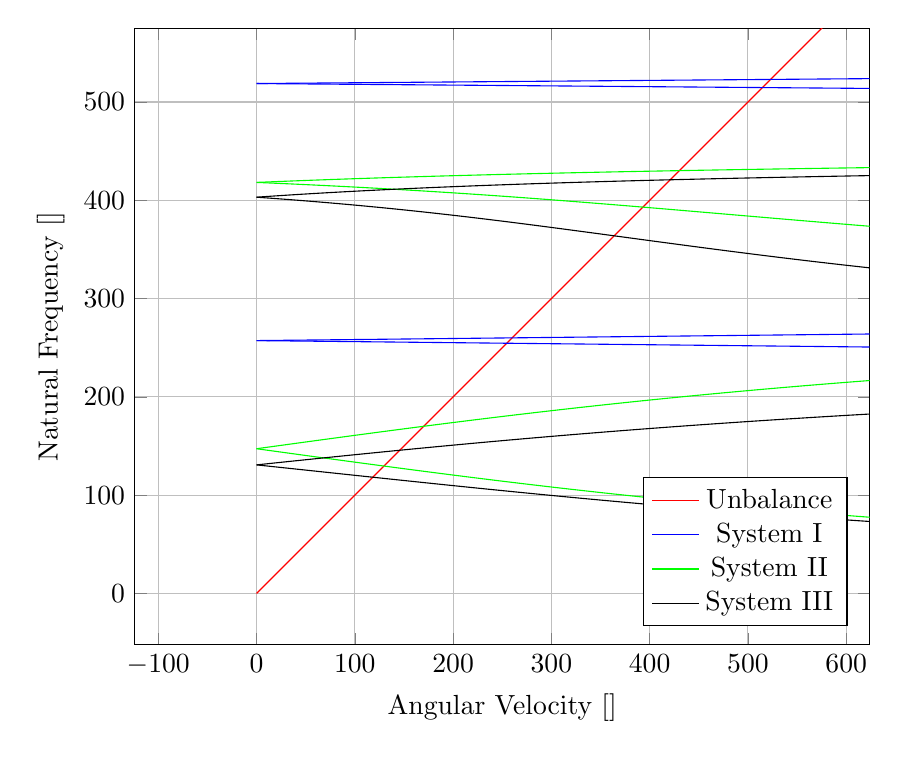
\begin{tikzpicture}
\begin{axis}[%
width=0.9\linewidth,
%height=0.9\linewidth,
xmax=500,
xmin=0,
xlabel={Angular Velocity [\si{\hertz}]},
ylabel={Natural Frequency [\si{\hertz}]},
grid=major,
legend pos=south east,
axis equal,
]
\addplot [color=red]
  table[row sep=crcr]{%
0	0\\
5	5\\
10	10\\
15	15\\
20	20\\
25	25\\
30	30\\
35	35\\
40	40\\
45	45\\
50	50\\
55	55\\
60	60\\
65	65\\
70	70\\
75	75\\
80	80\\
85	85\\
90	90\\
95	95\\
100	100\\
105	105\\
110	110\\
115	115\\
120	120\\
125	125\\
130	130\\
135	135\\
140	140\\
145	145\\
150	150\\
155	155\\
160	160\\
165	165\\
170	170\\
175	175\\
180	180\\
185	185\\
190	190\\
195	195\\
200	200\\
205	205\\
210	210\\
215	215\\
220	220\\
225	225\\
230	230\\
235	235\\
240	240\\
245	245\\
250	250\\
255	255\\
260	260\\
265	265\\
270	270\\
275	275\\
280	280\\
285	285\\
290	290\\
295	295\\
300	300\\
305	305\\
310	310\\
315	315\\
320	320\\
325	325\\
330	330\\
335	335\\
340	340\\
345	345\\
350	350\\
355	355\\
360	360\\
365	365\\
370	370\\
375	375\\
380	380\\
385	385\\
390	390\\
395	395\\
400	400\\
405	405\\
410	410\\
415	415\\
420	420\\
425	425\\
430	430\\
435	435\\
440	440\\
445	445\\
450	450\\
455	455\\
460	460\\
465	465\\
470	470\\
475	475\\
480	480\\
485	485\\
490	490\\
495	495\\
500	500\\
505	505\\
510	510\\
515	515\\
520	520\\
525	525\\
530	530\\
535	535\\
540	540\\
545	545\\
550	550\\
555	555\\
560	560\\
565	565\\
570	570\\
575	575\\
580	580\\
585	585\\
590	590\\
595	595\\
600	600\\
605	605\\
610	610\\
615	615\\
620	620\\
625	625\\
630	630\\
635	635\\
640	640\\
645	645\\
650	650\\
655	655\\
660	660\\
665	665\\
670	670\\
675	675\\
680	680\\
685	685\\
690	690\\
695	695\\
700	700\\
705	705\\
710	710\\
715	715\\
720	720\\
725	725\\
730	730\\
735	735\\
740	740\\
745	745\\
};
\addlegendentry{Unbalance}

\addplot [color=blue]
  table[row sep=crcr]{%
0	257.272586991077\\
5	257.216756305163\\
10	257.166122314727\\
15	257.115113452385\\
20	257.060285088651\\
25	257.006790700351\\
30	256.953798539078\\
35	256.900706325953\\
40	256.847882348684\\
45	256.794879138477\\
50	256.742532382384\\
55	256.689223408172\\
60	256.635850618845\\
65	256.583058553164\\
70	256.530018642645\\
75	256.47699236764\\
80	256.424003816099\\
85	256.371086173661\\
90	256.318116876878\\
95	256.265263191479\\
100	256.212319765853\\
105	256.159394682353\\
110	256.106752104767\\
115	256.053904622839\\
120	256.001041150304\\
125	255.948179779131\\
130	255.895431240398\\
135	255.842572540307\\
140	255.789661495036\\
145	255.736877230452\\
150	255.683959418278\\
155	255.631219413459\\
160	255.578409877976\\
165	255.525595660325\\
170	255.472849380452\\
175	255.420032040628\\
180	255.367247823351\\
185	255.314557456\\
190	255.261824507237\\
195	255.209027533111\\
200	255.156337577049\\
205	255.103646916983\\
210	255.05097839932\\
215	254.998312161035\\
220	254.945601851016\\
225	254.89291431462\\
230	254.840222127444\\
235	254.787605105338\\
240	254.73493260357\\
245	254.682319127622\\
250	254.629667800461\\
255	254.576984844884\\
260	254.524359435086\\
265	254.471844001447\\
270	254.419224724266\\
275	254.36665612185\\
280	254.314119482326\\
285	254.261582356509\\
290	254.209060912088\\
295	254.156497885873\\
300	254.103917115442\\
305	254.051426738989\\
310	253.998890147311\\
315	253.946435423718\\
320	253.893967788625\\
325	253.841492125426\\
330	253.788963802845\\
335	253.736492205133\\
340	253.684076970925\\
345	253.631700556921\\
350	253.579199966467\\
355	253.526812832744\\
360	253.474305751572\\
365	253.42198545965\\
370	253.369589224185\\
375	253.317210879281\\
380	253.264804116779\\
385	253.212472339583\\
390	253.16015523988\\
395	253.107793817576\\
400	253.055450943874\\
405	253.003114728444\\
410	252.950783914853\\
415	252.898505482253\\
420	252.846201228413\\
425	252.793908633072\\
430	252.74162843635\\
435	252.689403058539\\
440	252.63709690339\\
445	252.584841969055\\
450	252.53265104473\\
455	252.480423980978\\
460	252.428225846147\\
465	252.376023952813\\
470	252.323783055811\\
475	252.271581465921\\
480	252.219446918785\\
485	252.167281918348\\
490	252.115116109234\\
495	252.062986545162\\
500	252.010818678475\\
505	251.958701019062\\
510	251.906588852122\\
515	251.854491409917\\
520	251.80238160639\\
525	251.750276248531\\
530	251.698228550162\\
535	251.646125626471\\
540	251.594063256866\\
545	251.542032218959\\
550	251.489974349878\\
555	251.43796467612\\
560	251.385925740567\\
565	251.333893372762\\
570	251.281886309016\\
575	251.229975567328\\
580	251.177919587345\\
585	251.125961961362\\
590	251.074027360075\\
595	251.022048319568\\
600	250.970120457379\\
605	250.918198835664\\
610	250.866280950737\\
615	250.814339414972\\
620	250.762468557909\\
625	250.710594434505\\
630	250.658660864527\\
635	250.606825572877\\
640	250.554973768381\\
645	250.503079748869\\
650	250.4512487828\\
655	250.399394117994\\
660	250.347593152592\\
665	250.295742301692\\
670	250.243950719676\\
675	250.192169572187\\
680	250.140362795618\\
685	250.088615974885\\
690	250.036825857548\\
695	249.985083794921\\
700	249.933315581399\\
705	249.881633481997\\
710	249.829863184676\\
715	249.77814613184\\
720	249.726446144214\\
725	249.674741992092\\
730	249.623055710882\\
735	249.571388361496\\
740	249.519696356051\\
745	249.468024828992\\
};
\addlegendentry{System I}

\addplot [color=blue, forget plot]
  table[row sep=crcr]{%
0	257.272586991678\\
5	257.32318875337\\
10	257.378520396871\\
15	257.433736022089\\
20	257.485082668883\\
25	257.537785769627\\
30	257.590992830365\\
35	257.644100233949\\
40	257.69747405442\\
45	257.750670246285\\
50	257.804527292591\\
55	257.857414814236\\
60	257.910238207089\\
65	257.963648275598\\
70	258.016805617063\\
75	258.069976641877\\
80	258.123186267204\\
85	258.176468491851\\
90	258.229694872041\\
95	258.28304079911\\
100	258.336296219102\\
105	258.38956981736\\
110	258.443132287204\\
115	258.496484122984\\
120	258.549818154693\\
125	258.603156043906\\
130	258.656608235401\\
135	258.709947265627\\
140	258.763232444281\\
145	258.816648674979\\
150	258.869924916958\\
155	258.923386651969\\
160	258.976773695564\\
165	259.030157146567\\
170	259.083608721162\\
175	259.136986770483\\
180	259.19039917147\\
185	259.243907688037\\
190	259.297372149763\\
195	259.350771063142\\
200	259.404278819459\\
205	259.45778662604\\
210	259.511314527084\\
215	259.564845236061\\
220	259.618332381135\\
225	259.671840430029\\
230	259.725343785915\\
235	259.778922402504\\
240	259.83244551418\\
245	259.88602850883\\
250	259.939556719227\\
255	259.993066347048\\
260	260.046635473117\\
265	260.10031761741\\
270	260.153890913211\\
275	260.207517376141\\
280	260.261175014517\\
285	260.314831289872\\
290	260.368519424466\\
295	260.422146697615\\
300	260.475744325985\\
305	260.529446100188\\
310	260.583102043708\\
315	260.636841735359\\
320	260.690567820785\\
325	260.744284730834\\
330	260.797944116262\\
335	260.85166473043\\
340	260.9054416642\\
345	260.959260363744\\
350	261.012946670578\\
355	261.066751700558\\
360	261.12042964918\\
365	261.174303930184\\
370	261.228096292745\\
375	261.281907386223\\
380	261.335689001881\\
385	261.389548417645\\
390	261.443421736652\\
395	261.497247942817\\
400	261.551092425887\\
405	261.604942963693\\
410	261.658797908255\\
415	261.712708875078\\
420	261.766592755772\\
425	261.820485086567\\
430	261.874390681818\\
435	261.928355179252\\
440	261.982229879735\\
445	262.036160454569\\
450	262.0901564329\\
455	262.144115206768\\
460	262.198102888742\\
465	262.252087013453\\
470	262.306025810245\\
475	262.360007115338\\
480	262.414058894589\\
485	262.468077629632\\
490	262.522092511554\\
495	262.576147241797\\
500	262.630159227649\\
505	262.684224406054\\
510	262.738293755012\\
515	262.792378248858\\
520	262.846448070927\\
525	262.900522489443\\
530	262.954656590078\\
535	263.008729460318\\
540	263.062847945203\\
545	263.116996733271\\
550	263.171114032988\\
555	263.225285797228\\
560	263.279422070553\\
565	263.333562990593\\
570	263.387734778904\\
575	263.442006481675\\
580	263.496120732853\\
585	263.55033938918\\
590	263.604582382794\\
595	263.658776244684\\
600	263.713023326611\\
605	263.767278014891\\
610	263.821535648101\\
615	263.875762736236\\
620	263.930068931748\\
625	263.984368829717\\
630	264.038601594424\\
635	264.09294135351\\
640	264.147261213319\\
645	264.201534635613\\
650	264.255874779487\\
655	264.310188277114\\
660	264.364557924818\\
665	264.418873174279\\
670	264.473248815248\\
675	264.527639153555\\
680	264.581996035901\\
685	264.636421157372\\
690	264.690793360841\\
695	264.745218948886\\
700	264.799614775185\\
705	264.854102959176\\
710	264.908491749726\\
715	264.962938600759\\
720	265.017402632613\\
725	265.071861741121\\
730	265.126339144609\\
735	265.180833437148\\
740	265.235300632998\\
745	265.28978661919\\
};
\addplot [color=blue, forget plot]
  table[row sep=crcr]{%
0	518.821665977453\\
5	518.78558453498\\
10	518.741514550627\\
15	518.700751312816\\
20	518.659852156303\\
25	518.620042397766\\
30	518.580270986675\\
35	518.540870738576\\
40	518.50077036672\\
45	518.461011139881\\
50	518.422040908847\\
55	518.381859106328\\
60	518.342349590047\\
65	518.301686858617\\
70	518.261788576499\\
75	518.221972889584\\
80	518.182107620019\\
85	518.142103527475\\
90	518.102256206976\\
95	518.062159787043\\
100	518.022301292406\\
105	517.982414511259\\
110	517.943269733785\\
115	517.90327501769\\
120	517.863317873793\\
125	517.823393043221\\
130	517.783500985608\\
135	517.743526941726\\
140	517.703283465541\\
145	517.663319677564\\
150	517.623724691199\\
155	517.583696076342\\
160	517.543860584638\\
165	517.504029401468\\
170	517.464075436581\\
175	517.424307526636\\
180	517.384477921139\\
185	517.344443267144\\
190	517.304527127367\\
195	517.264807224166\\
200	517.224831581256\\
205	517.184885260127\\
210	517.144901411533\\
215	517.104944868159\\
220	517.065125442707\\
225	517.025261512638\\
230	516.985446971159\\
235	516.945467093764\\
240	516.905641120994\\
245	516.86570347409\\
250	516.825637379609\\
255	516.785906913326\\
260	516.746073105567\\
265	516.705977492349\\
270	516.666168293412\\
275	516.626251833317\\
280	516.586414092721\\
285	516.546447741534\\
290	516.506577557585\\
295	516.466775628609\\
300	516.426597388137\\
305	516.386674699898\\
310	516.346878509292\\
315	516.307029060585\\
320	516.267083192251\\
325	516.227190693619\\
330	516.187458364281\\
335	516.147607978865\\
340	516.10764442683\\
345	516.067590203371\\
350	516.027896085392\\
355	515.987932666367\\
360	515.94828949868\\
365	515.908199656497\\
370	515.868343993342\\
375	515.828452819239\\
380	515.788665016504\\
385	515.748716428428\\
390	515.708751888374\\
395	515.66891613624\\
400	515.6290676741\\
405	515.589231943915\\
410	515.549401352133\\
415	515.509474395464\\
420	515.469618949079\\
425	515.429770767964\\
430	515.389913872064\\
435	515.349946927465\\
440	515.310203379067\\
445	515.270361216757\\
450	515.230380554287\\
455	515.190524367992\\
460	515.150608790909\\
465	515.11073989488\\
470	515.070974460166\\
475	515.031147978421\\
480	514.991180919872\\
485	514.951314509181\\
490	514.911468885121\\
495	514.871565381276\\
500	514.831789003052\\
505	514.791893311319\\
510	514.752019171346\\
515	514.712133318357\\
520	514.672303788986\\
525	514.63249220188\\
530	514.592550289604\\
535	514.552785719906\\
540	514.51293392399\\
545	514.473036023459\\
550	514.433222933524\\
555	514.393320660539\\
560	514.353514521255\\
565	514.313717531102\\
570	514.273881715408\\
575	514.233832192074\\
580	514.194170349703\\
585	514.154286028785\\
590	514.114377695127\\
595	514.074590111562\\
600	514.03471283684\\
605	513.994843098689\\
610	513.954983093407\\
615	513.915210401837\\
620	513.87528072888\\
625	513.835393885634\\
630	513.795687993028\\
635	513.755749746744\\
640	513.715873631395\\
645	513.676131905172\\
650	513.636270773673\\
655	513.59648167198\\
660	513.556582967559\\
665	513.516844056985\\
670	513.476969678335\\
675	513.437102881036\\
680	513.397326252617\\
685	513.357415037909\\
690	513.317549307736\\
695	513.277682425144\\
700	513.237916873851\\
705	513.197953585915\\
710	513.158245250987\\
715	513.118428995463\\
720	513.078579743249\\
725	513.038778950939\\
730	512.998953008496\\
735	512.959108670901\\
740	512.919348133546\\
745	512.8795709902\\
};
\addplot [color=blue, forget plot]
  table[row sep=crcr]{%
0	518.821665977702\\
5	518.865507567108\\
10	518.901276110817\\
15	518.940644423583\\
20	518.97938094363\\
25	519.019432039367\\
30	519.059525625568\\
35	519.099998158819\\
40	519.139769619993\\
45	519.179881681912\\
50	519.220788866453\\
55	519.26047937891\\
60	519.300847868392\\
65	519.340052477696\\
70	519.380027651246\\
75	519.420088287963\\
80	519.460098474768\\
85	519.499966575482\\
90	519.539996544418\\
95	519.579772635221\\
100	519.61978901693\\
105	519.659773914085\\
110	519.700499868828\\
115	519.740378005554\\
120	519.78029738673\\
125	519.820245006711\\
130	519.860225552847\\
135	519.900125740357\\
140	519.939756117359\\
145	519.979663623156\\
150	520.019947185045\\
155	520.059788094977\\
160	520.09982791398\\
165	520.139870755099\\
170	520.179791003693\\
175	520.219896643281\\
180	520.259942529903\\
185	520.299780418661\\
190	520.339738195887\\
195	520.379892907511\\
200	520.419789958499\\
205	520.459715175477\\
210	520.499606189102\\
215	520.539522166004\\
220	520.579575023081\\
225	520.619585736787\\
230	520.659644930623\\
235	520.699538886211\\
240	520.739586836913\\
245	520.779520589816\\
250	520.819329004499\\
255	520.859472010869\\
260	520.899511920336\\
265	520.939287148447\\
270	520.979351216656\\
275	521.01930655894\\
280	521.05934412891\\
285	521.099249376058\\
290	521.139250155391\\
295	521.179324986162\\
300	521.219014060118\\
305	521.258967328999\\
310	521.299042029393\\
315	521.339067046927\\
320	521.378990963227\\
325	521.418970992593\\
330	521.459114413768\\
335	521.499134437715\\
340	521.539044241911\\
345	521.578858067317\\
350	521.619039234504\\
355	521.658947394017\\
360	521.699179689079\\
365	521.738957978982\\
370	521.778976426533\\
375	521.818956995386\\
380	521.859040837224\\
385	521.89896197308\\
390	521.938867522723\\
395	521.978904807318\\
400	522.018928176801\\
405	522.05896466705\\
410	522.09900665932\\
415	522.138951281786\\
420	522.178963830507\\
425	522.218988924671\\
430	522.25900383048\\
435	522.298905343817\\
440	522.339035605014\\
445	522.379065208487\\
450	522.418953683062\\
455	522.458968071637\\
460	522.498923284524\\
465	522.538923086479\\
470	522.579030187433\\
475	522.619074860438\\
480	522.658977328796\\
485	522.698978978444\\
490	522.739006079917\\
495	522.778970886861\\
500	522.819066010633\\
505	522.859038901296\\
510	522.899033797409\\
515	522.939017738097\\
520	522.979058868705\\
525	523.019115415391\\
530	523.059042814273\\
535	523.099149778818\\
540	523.13916559565\\
545	523.179136617646\\
550	523.219195151587\\
555	523.259159657842\\
560	523.299222616269\\
565	523.339299131266\\
570	523.379328889173\\
575	523.419145536941\\
580	523.459354821025\\
585	523.499338377764\\
590	523.539298675404\\
595	523.579378425806\\
600	523.619369742251\\
605	523.659366256801\\
610	523.699370951295\\
615	523.739470845206\\
620	523.779405499069\\
625	523.819384615964\\
630	523.859550112616\\
635	523.899476655875\\
640	523.939468214364\\
645	523.979594055705\\
650	524.019600903437\\
655	524.059677957022\\
660	524.099646565406\\
665	524.139774878142\\
670	524.179770613543\\
675	524.21976546784\\
680	524.259859727207\\
685	524.299807923306\\
690	524.339809043382\\
695	524.379807237106\\
700	524.419907596664\\
705	524.459807280264\\
710	524.499969047814\\
715	524.540018454664\\
720	524.580034050728\\
725	524.62009865794\\
730	524.660135188494\\
735	524.700156968001\\
740	524.740262595971\\
745	524.780353972661\\
};
\addplot [color=green]
  table[row sep=crcr]{%
0	147.243635606529\\
5	146.556929034497\\
10	145.870226144453\\
15	145.183565480321\\
20	144.497020772435\\
25	143.810653460489\\
30	143.124560753936\\
35	142.438784449493\\
40	141.753448022229\\
45	141.068505041038\\
50	140.384256707839\\
55	139.700649142517\\
60	139.0177084055\\
65	138.335479520391\\
70	137.654171987065\\
75	136.973736051567\\
80	136.294372434826\\
85	135.615957260473\\
90	134.938703399124\\
95	134.262640368648\\
100	133.587863921073\\
105	132.914432581398\\
110	132.242380212444\\
115	131.571805410464\\
120	130.902733163032\\
125	130.235255901257\\
130	129.569471292244\\
135	128.905347389691\\
140	128.243058533374\\
145	127.58260478703\\
150	126.92403169731\\
155	126.267398970743\\
160	125.612795655613\\
165	124.960256062301\\
170	124.30983173035\\
175	123.66159272741\\
180	123.01557186772\\
185	122.371812565112\\
190	121.730372045947\\
195	121.091360089192\\
200	120.454744510771\\
205	119.820566146531\\
210	119.18892021048\\
215	118.559837265263\\
220	117.933347164506\\
225	117.309468669867\\
230	116.688301774829\\
235	116.069827701973\\
240	115.454141560758\\
245	114.841201434232\\
250	114.231093022464\\
255	113.623849706979\\
260	113.019488808523\\
265	112.418044247496\\
270	111.819545913117\\
275	111.224009628654\\
280	110.631492107925\\
285	110.041989076696\\
290	109.455530878174\\
295	108.872135928363\\
300	108.291854455186\\
305	107.71468446405\\
310	107.140644299746\\
315	106.569760130946\\
320	106.00204113708\\
325	105.43750543642\\
330	104.876169530755\\
335	104.318043367474\\
340	103.763146071133\\
345	103.211492044891\\
350	102.663086074237\\
355	102.117917728489\\
360	101.576028464366\\
365	101.037407963788\\
370	100.502064133367\\
375	99.9700070812725\\
380	99.4412376133965\\
385	98.9157569064249\\
390	98.3935794563024\\
395	97.8746876165648\\
400	97.3590984767039\\
405	96.8468090905265\\
410	96.3378111505528\\
415	95.8321120812699\\
420	95.3297051513636\\
425	94.8305907938342\\
430	94.3347613008163\\
435	93.8422113327983\\
440	93.3529393260448\\
445	92.8669409357996\\
450	92.3842111342971\\
455	91.9047339445616\\
460	91.4285060333275\\
465	90.9555258044782\\
470	90.485772852519\\
475	90.0192442616835\\
480	89.5559308587307\\
485	89.0958272421979\\
490	88.6389089474763\\
495	88.1851740535295\\
500	87.7346092252898\\
505	87.2872028916842\\
510	86.842940734763\\
515	86.4018131124755\\
520	85.9638039339654\\
525	85.5288988434159\\
530	85.0970853502923\\
535	84.6683474152265\\
540	84.2426702490239\\
545	83.8200428239067\\
550	83.4004447658437\\
555	82.9838613616171\\
560	82.5702801150373\\
565	82.1596819027643\\
570	81.7520506771562\\
575	81.3473699243088\\
580	80.9456251517408\\
585	80.5467926326406\\
590	80.1508647623674\\
595	79.7578156416532\\
600	79.3676343384703\\
605	78.9802982299195\\
610	78.5957915103441\\
615	78.2140981813318\\
620	77.8351967737321\\
625	77.4590712745137\\
630	77.0857023393728\\
635	76.7150725578415\\
640	76.3471609266898\\
645	75.9819535634827\\
650	75.6194274017191\\
655	75.2595675787181\\
660	74.9023528811955\\
665	74.5477654054762\\
670	74.1957859513432\\
675	73.8463956807976\\
680	73.4995773310182\\
685	73.1553109224073\\
690	72.8135778479752\\
695	72.4743593053272\\
700	72.1376368061668\\
705	71.8033901241329\\
710	71.4716021603126\\
715	71.1422544183783\\
720	70.8153267804997\\
725	70.490801091945\\
730	70.1686602420114\\
735	69.8488834433355\\
740	69.5314537540011\\
745	69.2163510003807\\
};
\addlegendentry{System II}

\addplot [color=green, forget plot]
  table[row sep=crcr]{%
0	147.243635606758\\
5	147.930193998975\\
10	148.61660943431\\
15	149.302771611007\\
20	149.988607334787\\
25	150.674029885481\\
30	151.358993233954\\
35	152.043387653956\\
40	152.72719884439\\
45	153.410215201274\\
50	154.092631185835\\
55	154.774234842691\\
60	155.454897068255\\
65	156.13451019951\\
70	156.813183514079\\
75	157.490692800356\\
80	158.167139266229\\
85	158.842206899974\\
90	159.516014448534\\
95	160.188445554438\\
100	160.859476677991\\
105	161.529037074486\\
110	162.19701305804\\
115	162.863395100759\\
120	163.528061135981\\
125	164.190996512224\\
130	164.852204175635\\
135	165.511476595918\\
140	166.168930899041\\
145	166.824428705411\\
150	167.477891759974\\
155	168.129266916242\\
160	168.778564833091\\
165	169.425697148933\\
170	170.070609506263\\
175	170.713286103856\\
180	171.353648666987\\
185	171.991633192236\\
190	172.627208462206\\
195	173.260470856939\\
200	173.891214357555\\
205	174.519364808565\\
210	175.145018756456\\
215	175.768105809976\\
220	176.388561468548\\
225	177.006295479241\\
230	177.621425400787\\
235	178.233778224805\\
240	178.84347269604\\
245	179.450279928305\\
250	180.054304531576\\
255	180.655519967306\\
260	181.253866192436\\
265	181.849328808358\\
270	182.44188131747\\
275	183.03146996772\\
280	183.618163331813\\
285	184.201853233733\\
290	184.782540263491\\
295	185.360190169164\\
300	185.934880480738\\
305	186.506523878128\\
310	187.07510158013\\
315	187.640630227451\\
320	188.203068371845\\
325	188.76241660836\\
330	189.318668063937\\
335	189.871801055301\\
340	190.421833093628\\
345	190.968769019652\\
350	191.512582426847\\
355	192.053189373125\\
360	192.590721996159\\
365	193.125093046335\\
370	193.65631495243\\
375	194.184405416071\\
380	194.709346635953\\
385	195.231128901969\\
390	195.749805163203\\
395	196.265289837601\\
400	196.777659707154\\
405	197.286903339837\\
410	197.792979646086\\
415	198.295947208029\\
420	198.795783180799\\
425	199.292512657544\\
430	199.786121056651\\
435	200.276605901265\\
440	200.763995308646\\
445	201.248307603602\\
450	201.729557912351\\
455	202.207706858847\\
460	202.682777558576\\
465	203.154833376918\\
470	203.62380188182\\
475	204.089737928167\\
480	204.552659988592\\
485	205.012612607045\\
490	205.469506053091\\
495	205.923427811069\\
500	206.374377267556\\
505	206.822367984245\\
510	207.267404880539\\
515	207.709523290941\\
520	208.148719010118\\
525	208.585002127522\\
530	209.018396827578\\
535	209.44890942241\\
540	209.876551838631\\
545	210.301371824871\\
550	210.723344761104\\
555	211.142493784685\\
560	211.558862531998\\
565	211.972441067058\\
570	212.383253221305\\
575	212.791310963491\\
580	213.196651775148\\
585	213.599236678193\\
590	213.999162177825\\
595	214.396372973348\\
600	214.790944164611\\
605	215.18284713185\\
610	215.572118021545\\
615	215.958793464173\\
620	216.342856597386\\
625	216.724346606834\\
630	217.103270464343\\
635	217.479655371896\\
640	217.853491236596\\
645	218.224843230015\\
650	218.593684858253\\
655	218.960069155425\\
660	219.323991707111\\
665	219.685476224512\\
670	220.044533842354\\
675	220.401184218417\\
680	220.755459050193\\
685	221.107364657455\\
690	221.456920766256\\
695	221.804144687453\\
700	222.149056427138\\
705	222.491657558007\\
710	222.831984075107\\
715	223.170057926412\\
720	223.505877177927\\
725	223.839464709575\\
730	224.170860006015\\
735	224.500051409857\\
740	224.827078899775\\
745	225.151924868536\\
};
\addplot [color=green, forget plot]
  table[row sep=crcr]{%
0	418.208170844837\\
5	417.996240190607\\
10	417.780752339464\\
15	417.563490504093\\
20	417.343616735382\\
25	417.121410397931\\
30	416.896740821938\\
35	416.669403110155\\
40	416.439518844835\\
45	416.207075598458\\
50	415.972071517441\\
55	415.734148793872\\
60	415.493710402879\\
65	415.250783431045\\
70	415.004881488608\\
75	414.756432519737\\
80	414.505151071216\\
85	414.251000604269\\
90	413.994128713516\\
95	413.734478721729\\
100	413.47190384116\\
105	413.206400319661\\
110	412.938092858449\\
115	412.66682729699\\
120	412.392757399501\\
125	412.115710160731\\
130	411.835513482911\\
135	411.55247530664\\
140	411.266450418003\\
145	410.977419019596\\
150	410.685368261685\\
155	410.390370469031\\
160	410.092264327137\\
165	409.791136330592\\
170	409.487036763035\\
175	409.17978984153\\
180	408.869508433576\\
185	408.556315209345\\
190	408.240087526208\\
195	407.920539972447\\
200	407.598209537647\\
205	407.272790220232\\
210	406.94434079625\\
215	406.612857790779\\
220	406.278415567288\\
225	405.941085311674\\
230	405.600614366269\\
235	405.257337586214\\
240	404.910912912451\\
245	404.561821552384\\
250	404.209821184792\\
255	403.854836378601\\
260	403.497077604144\\
265	403.13659094052\\
270	402.773250970069\\
275	402.407270043357\\
280	402.038470615599\\
285	401.667106166417\\
290	401.293156019042\\
295	400.916703232638\\
300	400.537595262169\\
305	400.156032729006\\
310	399.772071138714\\
315	399.385702694091\\
320	398.997024829567\\
325	398.60609933713\\
330	398.212946272431\\
335	397.817660335719\\
340	397.420252799767\\
345	397.020770062713\\
350	396.619298954207\\
355	396.216051618409\\
360	395.810902661543\\
365	395.403939192083\\
370	394.995280506915\\
375	394.58496309545\\
380	394.173073592031\\
385	393.759710167891\\
390	393.344838239258\\
395	392.928694462843\\
400	392.511218356362\\
405	392.092521691475\\
410	391.672687144709\\
415	391.251774203796\\
420	390.829865553969\\
425	390.407013143399\\
430	389.983325316669\\
435	389.558873424849\\
440	389.13370552198\\
445	388.707895925824\\
450	388.281494764845\\
455	387.854669932161\\
460	387.42740329039\\
465	386.999777616579\\
470	386.571904842649\\
475	386.14381690024\\
480	385.71560167984\\
485	385.2873252747\\
490	384.859049844325\\
495	384.430834380087\\
500	384.002762299715\\
505	383.57488634104\\
510	383.147284988877\\
515	382.719985806896\\
520	382.29308863697\\
525	381.866647412062\\
530	381.440710899331\\
535	381.015346762999\\
540	380.590614374444\\
545	380.16653650169\\
550	379.743206640942\\
555	379.32066961895\\
560	378.898951339785\\
565	378.4781947443\\
570	378.058234178723\\
575	377.639327352106\\
580	377.221432737435\\
585	376.80464715757\\
590	376.38893638239\\
595	375.974411873878\\
600	375.561060094338\\
605	375.148960909394\\
610	374.738134285192\\
615	374.328602295889\\
620	373.920425441472\\
625	373.513621711706\\
630	373.10823079207\\
635	372.704279968678\\
640	372.301811986563\\
645	371.900823675737\\
650	371.501375372379\\
655	371.103466306868\\
660	370.707137182389\\
665	370.312407909918\\
670	369.919304789798\\
675	369.52784787863\\
680	369.138047073888\\
685	368.749929422098\\
690	368.363512185017\\
695	367.978812216369\\
700	367.595842122415\\
705	367.214628096035\\
710	366.835144018613\\
715	366.457454645964\\
720	366.08155758151\\
725	365.707459383202\\
730	365.335160652947\\
735	364.964684634748\\
740	364.59603461422\\
745	364.22921546498\\
};
\addplot [color=green, forget plot]
  table[row sep=crcr]{%
0	418.208170845272\\
5	418.41887140035\\
10	418.626081847182\\
15	418.831621066071\\
20	419.034718386527\\
25	419.235704936555\\
30	419.434495560264\\
35	419.630965144434\\
40	419.825270184973\\
45	420.0174541993\\
50	420.207571918488\\
55	420.395315861471\\
60	420.581147275375\\
65	420.765140392903\\
70	420.946863557047\\
75	421.126775313835\\
80	421.304678655925\\
85	421.480561298864\\
90	421.654630401638\\
95	421.826868627833\\
100	421.997177812785\\
105	422.16559943307\\
110	422.332303842491\\
115	422.497181564994\\
120	422.660429278354\\
125	422.821906688305\\
130	422.981485528751\\
135	423.139520340162\\
140	423.295891613225\\
145	423.450622151415\\
150	423.603728106729\\
155	423.75531769991\\
160	423.905259014693\\
165	424.053664798422\\
170	424.200608346404\\
175	424.345952498843\\
180	424.489825719555\\
185	424.632377442358\\
190	424.773501657996\\
195	424.912914080641\\
200	425.051198364448\\
205	425.188036749266\\
210	425.32350776072\\
215	425.457618469591\\
220	425.590450799091\\
225	425.72208591634\\
230	425.852253221121\\
235	425.98131101284\\
240	426.108890494308\\
245	426.23549927227\\
250	426.360870747098\\
255	426.484910608384\\
260	426.607830538543\\
265	426.729669140242\\
270	426.850268182929\\
275	426.96984153855\\
280	427.088157474013\\
285	427.205483579333\\
290	427.321758713191\\
295	427.437049305027\\
300	427.551138907955\\
305	427.664221857793\\
310	427.776318865906\\
315	427.887375446245\\
320	427.997476821434\\
325	428.106620045038\\
330	428.214783603408\\
335	428.322026889602\\
340	428.42830804087\\
345	428.533621530796\\
350	428.638006560211\\
355	428.741662510215\\
360	428.844367236028\\
365	428.946158850507\\
370	429.047113118066\\
375	429.147202872802\\
380	429.246460399269\\
385	429.344938700219\\
390	429.442505264159\\
395	429.539394125202\\
400	429.635437036638\\
405	429.730699113703\\
410	429.825203690052\\
415	429.91894296858\\
420	430.011939286877\\
425	430.104174404886\\
430	430.195704752791\\
435	430.286540705745\\
440	430.376620973791\\
445	430.466055747281\\
450	430.554717820411\\
455	430.64278836685\\
460	430.730158788303\\
465	430.816833988771\\
470	430.90290606053\\
475	430.988318101042\\
480	431.073095331336\\
485	431.157228428865\\
490	431.240776721881\\
495	431.323681096155\\
500	431.405997023797\\
505	431.487708197435\\
510	431.568847718119\\
515	431.649368107176\\
520	431.729332252119\\
525	431.808741488912\\
530	431.887587501115\\
535	431.965894048876\\
540	432.043672668518\\
545	432.120873131594\\
550	432.197568696049\\
555	432.273758075952\\
560	432.349400600715\\
565	432.424629270453\\
570	432.499179398057\\
575	432.573323131467\\
580	432.646946554717\\
585	432.720165510855\\
590	432.792813049184\\
595	432.865056803405\\
600	432.936777059853\\
605	433.008075800207\\
610	433.07891640828\\
615	433.149273465815\\
620	433.219211813846\\
625	433.288700416782\\
630	433.357764199472\\
635	433.426385228576\\
640	433.494623444941\\
645	433.5623956215\\
650	433.629790832241\\
655	433.696745358938\\
660	433.763305815861\\
665	433.829466102129\\
670	433.895247467653\\
675	433.960644300999\\
680	434.025639683953\\
685	434.090254591802\\
690	434.154498571605\\
695	434.218369603048\\
700	434.281866380915\\
705	434.345028616292\\
710	434.407766626201\\
715	434.470178096842\\
720	434.532262094178\\
725	434.594006377939\\
730	434.655377046782\\
735	434.716429043975\\
740	434.777139473737\\
745	434.837527713762\\
};
\addplot [color=black]
  table[row sep=crcr]{%
0	130.803903895619\\
5	130.276573284169\\
10	129.748476992757\\
15	129.219876509548\\
20	128.690840106557\\
25	128.161055708166\\
30	127.630943489819\\
35	127.100463761011\\
40	126.569621479213\\
45	126.03848042\\
50	125.507201653895\\
55	124.975750153557\\
60	124.444057054387\\
65	123.912307815972\\
70	123.380524403987\\
75	122.848785714771\\
80	122.317114745439\\
85	121.785557008025\\
90	121.254166243174\\
95	120.723031906455\\
100	120.192146539641\\
105	119.661626005079\\
110	119.131436010311\\
115	118.601697085719\\
120	118.072449562586\\
125	117.543719167486\\
130	117.015581903537\\
135	116.488053120412\\
140	115.961222494416\\
145	115.435134447831\\
150	114.909799798545\\
155	114.385281894818\\
160	113.861621867336\\
165	113.338905863959\\
170	112.817132184315\\
175	112.296362581399\\
180	111.776677212688\\
185	111.258085865506\\
190	110.740597575528\\
195	110.224351169728\\
200	109.709315736712\\
205	109.195508990753\\
210	108.683041987936\\
215	108.171938075671\\
220	107.662204790531\\
225	107.153913456389\\
230	106.647104921076\\
235	106.141783236123\\
240	105.638026099803\\
245	105.135822564585\\
250	104.635257709053\\
255	104.136330189039\\
260	103.639079735629\\
265	103.143561776671\\
270	102.649776819824\\
275	102.157780111697\\
280	101.667581876676\\
285	101.179231351348\\
290	100.692727431587\\
295	100.208138224701\\
300	99.7254918976935\\
305	99.2447716150982\\
310	98.7660192553957\\
315	98.2892703416997\\
320	97.8145453797171\\
325	97.3418665090394\\
330	96.8712487614912\\
335	96.4027221430597\\
340	95.936291456148\\
345	95.4719975276023\\
350	95.0098522597937\\
355	94.5498715177542\\
360	94.0920629200549\\
365	93.6364563201433\\
370	93.1830464563343\\
375	92.7318705370307\\
380	92.2829411041461\\
385	91.8362668616714\\
390	91.3918470881858\\
395	90.949709861512\\
400	90.5098536487509\\
405	90.0722981504767\\
410	89.6370520475605\\
415	89.2041224229448\\
420	88.7735167731116\\
425	88.3452291649982\\
430	87.9192947236326\\
435	87.4956946879432\\
440	87.0744470057392\\
445	86.6555547493536\\
450	86.2390148600961\\
455	85.824838255745\\
460	85.4130227986783\\
465	85.0035790374145\\
470	84.5964981127788\\
475	84.1917851048689\\
480	83.7894423994916\\
485	83.3894739975056\\
490	82.991868345572\\
495	82.5966366129513\\
500	82.2037703738872\\
505	81.8132675244862\\
510	81.4251322731929\\
515	81.0393514093962\\
520	80.6559310100952\\
525	80.2748598902475\\
530	79.8961409708293\\
535	79.5197709914107\\
540	79.1457343855335\\
545	78.7740368243035\\
550	78.4046613072508\\
555	78.0376145253539\\
560	77.6728859565968\\
565	77.3104672656032\\
570	76.9503502036759\\
575	76.5925304977168\\
580	76.2369996148269\\
585	75.8837501342443\\
590	75.5327705119365\\
595	75.1840602772768\\
600	74.8375993395776\\
605	74.4933923999748\\
610	74.1514181991442\\
615	73.8116758881726\\
620	73.4741492556414\\
625	73.1388365535029\\
630	72.8057239503934\\
635	72.4747964222721\\
640	72.1460478580664\\
645	71.8194694428927\\
650	71.4950516213707\\
655	71.1727771850663\\
660	70.8526418207705\\
665	70.5346332107361\\
670	70.218735158267\\
675	69.9049455094481\\
680	69.5932397542301\\
685	69.2836179397042\\
690	68.9760614764057\\
695	68.6705657542979\\
700	68.3671123667637\\
705	68.0656917362538\\
710	67.7662918243856\\
715	67.4689010706449\\
720	67.1735058248694\\
725	66.8800970219982\\
730	66.5886597179132\\
735	66.2991810275753\\
740	66.0116496932902\\
745	65.7260554219829\\
};
\addlegendentry{System III}

\addplot [color=black, forget plot]
  table[row sep=crcr]{%
0	130.803903896033\\
5	131.330690962876\\
10	131.856614318957\\
15	132.381841214025\\
20	132.906349279923\\
25	133.429707120885\\
30	133.952260050874\\
35	134.473866587815\\
40	134.994437133056\\
45	135.513934140389\\
50	136.032434879865\\
55	136.549812145612\\
60	137.06587759837\\
65	137.58074469884\\
70	138.094337317583\\
75	138.606646789618\\
80	139.117602656334\\
85	139.62715455068\\
90	140.135268461166\\
95	140.641958098396\\
100	141.147106139101\\
105	141.650768138938\\
110	142.152787356263\\
115	142.653229473975\\
120	143.152048541384\\
125	143.649173944809\\
130	144.14461580018\\
135	144.638280021748\\
140	145.130215668803\\
145	145.620383108735\\
150	146.108690734732\\
155	146.595135950015\\
160	147.079679969419\\
165	147.562368595976\\
170	148.043089829987\\
175	148.521850609566\\
180	148.998686185732\\
185	149.473517396045\\
190	149.946249465829\\
195	150.417052731529\\
200	150.885753796223\\
205	151.352299922612\\
210	151.816797925876\\
215	152.279204324622\\
220	152.739429976901\\
225	153.197530510551\\
230	153.653496708617\\
235	154.107241080663\\
240	154.558835583595\\
245	155.008166603892\\
250	155.455337217593\\
255	155.900249894426\\
260	156.342908511765\\
265	156.783361880929\\
270	157.22151979201\\
275	157.657435102668\\
280	158.091048193024\\
285	158.522408433172\\
290	158.951419928507\\
295	159.378194105046\\
300	159.802732014947\\
305	160.224904452218\\
310	160.644754522648\\
315	161.062313940528\\
320	161.477569097288\\
325	161.890518912359\\
330	162.301139026861\\
335	162.709457466141\\
340	163.115423702036\\
345	163.519108541654\\
350	163.920492309939\\
355	164.319567924605\\
360	164.716307770551\\
365	165.110760152164\\
370	165.502851899335\\
375	165.892670912751\\
380	166.280216551647\\
385	166.665475706719\\
390	167.048405577469\\
395	167.42907241894\\
400	167.807431299362\\
405	168.183529766253\\
410	168.557369090903\\
415	168.928950916666\\
420	169.298279174943\\
425	169.665301444574\\
430	170.030152748422\\
435	170.392728955497\\
440	170.753096074922\\
445	171.111255336919\\
450	171.467179436317\\
455	171.820912633423\\
460	172.172441548252\\
465	172.52181608387\\
470	172.868989720532\\
475	173.213993505292\\
480	173.556845197705\\
485	173.897576111098\\
490	174.236136029268\\
495	174.572601468695\\
500	174.906944101464\\
505	175.239172567079\\
510	175.569336366019\\
515	175.897382801046\\
520	176.223381964448\\
525	176.547295108259\\
530	176.869179236544\\
535	177.189053239434\\
540	177.506860038579\\
545	177.822680435818\\
550	178.136452165852\\
555	178.448270335362\\
560	178.758119480957\\
565	179.066000002756\\
570	179.371912617824\\
575	179.675891137577\\
580	179.977940098985\\
585	180.278076050323\\
590	180.576285858411\\
595	180.872638496193\\
600	181.167059335685\\
605	181.459667196648\\
610	181.750377878555\\
615	182.039269903345\\
620	182.32630699719\\
625	182.611555751036\\
630	182.895006525897\\
635	183.176628529426\\
640	183.456463429711\\
645	183.734546279258\\
650	184.010895055693\\
655	184.285460153619\\
660	184.558328434873\\
665	184.829480132775\\
670	185.098902691334\\
675	185.366659956984\\
680	185.632703223109\\
685	185.89709801101\\
690	186.159803278661\\
695	186.420899497879\\
700	186.68036187263\\
705	186.938191232102\\
710	187.194412883301\\
715	187.449043025791\\
720	187.70207722367\\
725	187.953561443488\\
730	188.203476938606\\
735	188.451829426034\\
740	188.698643840538\\
745	188.943956870723\\
};
\addplot [color=black, forget plot]
  table[row sep=crcr]{%
0	403.171424503726\\
5	402.820115671006\\
10	402.463899723504\\
15	402.102390667794\\
20	401.736068743526\\
25	401.36431534114\\
30	400.987438198565\\
35	400.605310745489\\
40	400.217837999288\\
45	399.824994368896\\
50	399.426627651883\\
55	399.022770704665\\
60	398.613386654043\\
65	398.198282564663\\
70	397.777567989739\\
75	397.351270373986\\
80	396.91908011217\\
85	396.481191724842\\
90	396.037608832101\\
95	395.587954076726\\
100	395.132637342163\\
105	394.671211451821\\
110	394.204144952438\\
115	393.731043656573\\
120	393.25195394217\\
125	392.766980068375\\
130	392.276017815954\\
135	391.779277640947\\
140	391.276459986903\\
145	390.767620522539\\
150	390.253017100706\\
155	389.732563086075\\
160	389.206345274049\\
165	388.674167817308\\
170	388.13635632241\\
175	387.592780799394\\
180	387.043510687054\\
185	386.488571541021\\
190	385.928342556933\\
195	385.362311562059\\
200	384.791089635597\\
205	384.214655909916\\
210	383.632900045058\\
215	383.04597347464\\
220	382.45414797854\\
225	381.857367857781\\
230	381.255705316952\\
235	380.64946064199\\
240	380.03861394151\\
245	379.423439828919\\
250	378.803856122774\\
255	378.180202522293\\
260	377.552570379944\\
265	376.920973240914\\
270	376.285746411417\\
275	375.646907687848\\
280	375.004739911026\\
285	374.359343502581\\
290	373.710977156881\\
295	373.059565752074\\
300	372.405306178588\\
305	371.748622557031\\
310	371.089585711369\\
315	370.428305910114\\
320	369.764972702946\\
325	369.099762775155\\
330	368.432886807505\\
335	367.764477464212\\
340	367.094789023364\\
345	366.423884392479\\
350	365.75195472926\\
355	365.079223276676\\
360	364.405877355356\\
365	363.732018772969\\
370	363.057937929265\\
375	362.383677405615\\
380	361.70937794916\\
385	361.0352496584\\
390	360.361519904291\\
395	359.688251056918\\
400	359.015663529004\\
405	358.343845437912\\
410	357.672950696369\\
415	357.003124478278\\
420	356.334516435551\\
425	355.667323827901\\
430	355.001531082447\\
435	354.337401924384\\
440	353.675028656427\\
445	353.01437712561\\
450	352.355774155416\\
455	351.69923732886\\
460	351.044894074735\\
465	350.392809827197\\
470	349.743132079099\\
475	349.095938085189\\
480	348.451308625531\\
485	347.809315795699\\
490	347.170092614712\\
495	346.533664668506\\
500	345.900138347493\\
505	345.269586028233\\
510	344.642049496191\\
515	344.01763539874\\
520	343.396367466829\\
525	342.778333802886\\
530	342.163560288671\\
535	341.552102091921\\
540	340.944068886422\\
545	340.339368779692\\
550	339.7381676064\\
555	339.140455859443\\
560	338.546270594263\\
565	337.955652107009\\
570	337.368633281539\\
575	336.785232512886\\
580	336.205478106914\\
585	335.629390460724\\
590	335.057000111545\\
595	334.488302828674\\
600	333.923344861416\\
605	333.362103853249\\
610	332.804622308239\\
615	332.25088904708\\
620	331.700924284729\\
625	331.154721590023\\
630	330.612288783535\\
635	330.073642924106\\
640	329.538763445445\\
645	329.007658595898\\
650	328.480319837266\\
655	327.956753689305\\
660	327.436951306424\\
665	326.920894471405\\
670	326.408588281911\\
675	325.90001755248\\
680	325.395177636231\\
685	324.894052262891\\
690	324.396632987894\\
695	323.902901463743\\
700	323.412846353679\\
705	322.926453347546\\
710	322.44370621134\\
715	321.964582926984\\
720	321.48908013958\\
725	321.017166341781\\
730	320.548818844856\\
735	320.084043863324\\
740	319.622795919381\\
745	319.165064342975\\
};
\addplot [color=black, forget plot]
  table[row sep=crcr]{%
0	403.171424504001\\
5	403.517866425882\\
10	403.859528831973\\
15	404.196161895155\\
20	404.528354985015\\
25	404.855649574052\\
30	405.178455604435\\
35	405.4967823631\\
40	405.810638254215\\
45	406.120149451482\\
50	406.425309145562\\
55	406.726202009613\\
60	407.022946591543\\
65	407.315456972108\\
70	407.603952468493\\
75	407.888571516853\\
80	408.169106355217\\
85	408.445856102313\\
90	408.71893362829\\
95	408.988013489802\\
100	409.253645579971\\
105	409.515421239113\\
110	409.773936665536\\
115	410.028838742835\\
120	410.280246740331\\
125	410.528340716246\\
130	410.773065570869\\
135	411.014736518362\\
140	411.25301656053\\
145	411.488025803306\\
150	411.720095428681\\
155	411.949147943309\\
160	412.175308862695\\
165	412.398353729929\\
170	412.618674406752\\
175	412.83609261747\\
180	413.050711911938\\
185	413.262505856287\\
190	413.471918062534\\
195	413.678279188036\\
200	413.88229088673\\
205	414.083879174876\\
210	414.282820401396\\
215	414.479242890321\\
220	414.67339856646\\
225	414.865134701712\\
230	415.054420348102\\
235	415.241546851346\\
240	415.426341548862\\
245	415.609078441183\\
250	415.789475622523\\
255	415.967856991726\\
260	416.14418535477\\
265	416.318311938213\\
270	416.490538862676\\
275	416.660699870414\\
280	416.82902369339\\
285	416.995321766098\\
290	417.159960620227\\
295	417.322561169107\\
300	417.483149494096\\
305	417.642162162481\\
310	417.799476529478\\
315	417.955014526804\\
320	418.108830416031\\
325	418.260955222701\\
330	418.411491938937\\
335	418.560375567758\\
340	418.707795076375\\
345	418.853556295715\\
350	418.997737950962\\
355	419.140411249679\\
360	419.281683569556\\
365	419.421429465712\\
370	419.559915710979\\
375	419.696918199891\\
380	419.83243143878\\
385	419.966560741151\\
390	420.099479474897\\
395	420.231014005824\\
400	420.361334912432\\
405	420.49033334468\\
410	420.618048184042\\
415	420.744520743387\\
420	420.869756492682\\
425	420.993972174744\\
430	421.116810771628\\
435	421.238620210059\\
440	421.359311699684\\
445	421.478702642806\\
450	421.59710710931\\
455	421.714420004569\\
460	421.830694994309\\
465	421.945847184797\\
470	422.060037462793\\
475	422.173234353836\\
480	422.285391326425\\
485	422.39650572625\\
490	422.506751908416\\
495	422.61595748331\\
500	422.724247370097\\
505	422.831637403603\\
510	422.938040833892\\
515	423.043636729359\\
520	423.148284100884\\
525	423.25212719378\\
530	423.355062471624\\
535	423.457093541914\\
540	423.558450210138\\
545	423.658799500584\\
550	423.758496674777\\
555	423.857317193533\\
560	423.955306555893\\
565	424.052574793149\\
570	424.149092696001\\
575	424.244769073516\\
580	424.339824680833\\
585	424.434105590872\\
590	424.52769939936\\
595	424.620529763021\\
600	424.712724202946\\
605	424.804119398136\\
610	424.894943937405\\
615	424.985072153744\\
620	425.074510879001\\
625	425.163277546948\\
630	425.251367701576\\
635	425.33898233341\\
640	425.425877068084\\
645	425.512162197953\\
650	425.597801318865\\
655	425.682887657352\\
660	425.767348051013\\
665	425.85121277081\\
670	425.934552846958\\
675	426.017263337855\\
680	426.099475555951\\
685	426.18109494511\\
690	426.262249707801\\
695	426.342782348326\\
700	426.422774455533\\
705	426.502283502697\\
710	426.581274292349\\
715	426.659736819002\\
720	426.737737256468\\
725	426.815182458035\\
730	426.892147341856\\
735	426.968688915914\\
740	427.044745592705\\
745	427.120272612166\\
};
\end{axis}

\end{tikzpicture}%
    \caption{Campbell diagram of system (I), (II) and (III)}
    \label{fig:campbell_diagram}
\end{figure}


\subsubsection{First mode shapes}
cfbcv
\subsection{Unbalance response}
cfbc
\section{Modelling of Hydrodynamic Bearing}
cfbcv
\subsection{Hydrodynamic bearing - Properties}
cvbf
\subsubsection{Assumptions}
xcbf
\subsubsection{External static load}
dfgv
\subsubsection{Oil film thickness}
gdrt
\subsubsection{Stiffnes and damping}
cvncn
\subsection{Prediction of Critical Speed}
dfg
\subsubsection{First two critical speeds}
hjkh
\subsubsection{Operational range}
fgj
\subsection{Rotor Bearing Stability Limit}
sdg
\subsubsection{Maximum angular velocity}
sdf
\subsubsection{Frequency of unstable vibration}
sdf
\subsubsection{Ratio between unstable Frequency and angular velocity}
ælkdsf
\subsection{Unbalance response}
sdf
\subsection{Engeineering application}
sdf
\subsubsection{Extend maximum angular velocity}
ælkaæslkæalskd
\subsubsection{Procentile improvement}
ælaksældk